\documentclass[table,serif,mathserif,final]{beamer}
\mode<presentation>{\usetheme{Lankton}}
\RequirePackage{ragged2e}
\usepackage{amsmath,amsfonts,amssymb,pxfonts,xspace}
\usepackage{graphicx}
\graphicspath{{./figures/}}
\usepackage[orientation=landscape,size=custom,width=50.8,height=76.2,scale=.4,debug]{beamerposter}
%\usepackage{pslatex} % use times roman
\usepackage{amsmath}
\usepackage{amssymb}
\usepackage{amsthm}
\usepackage{color}
\usepackage{array}
\usepackage{xy}
\usepackage{setspace}
\usepackage{tikz}
\usetikzlibrary{matrix}
\usepackage{mathptmx }
\usetikzlibrary{arrows,shapes}
\usepackage{pifont}
\newcommand{\cmark}{{\color{blue}\fontsize{65}{60}\selectfont \ding{51}}}%
\newcommand{\xmark}{{\color{red}\fontsize{65}{60}\selectfont \ding{55}}}%
\newcommand{\citefont}[1]{{\huge \textcolor{gray}{#1}}}


\usepackage[makeroom]{cancel}
\usepackage{verbatim}
\usetikzlibrary{arrows,shapes}


\newcommand*\mycirc[1]{%
  \begin{tikzpicture}
    \node[draw,circle,inner sep=1pt] {#1};
  \end{tikzpicture}}

\newcommand\iitem{\item[\begin{Large}$\bullet$\end{Large}]}

\newcommand{\rot}{\operatorname*{rot}}

%\usepackage[pdftex]{graphicx}
%\usepackage[left=1.5in,right=1.5in, top=1.5in,bottom=1.5in,]{geometry}
\newcommand{\edit}[1]{{\color{red}\textbf{#1}}}
\newcommand{\CC}{\mathbb{C}}
\newcommand{\NN}{\mathbb{N}}
\newcommand{\ZZ}{\mathbb{Z}}
\newcommand{\ot}{\otimes}
\newcommand{\sign}{\operatorname{sign}}

%----------------MACROS---------------%
\newtheorem{thm}{Theorem}[section]
\newtheorem{defn}[thm]{Definition}
\newtheorem{lem}[thm]{Lemma}
\newtheorem{prop}[thm]{Proposition}
\newtheorem{clm}[thm]{Claim} 
\newtheorem{cor}[thm]{Corollary}
\newtheorem{conj}[thm]{Conjecture}
\theoremstyle{remark}
\newtheorem{rem}[thm]{Remark}
\newtheorem{ex}[thm]{Example}

\newcommand{\mycenter}[1]{\hfil #1 \hfil}
\newcommand{\myzero}{\hfil $0$ \hfil}
\newcommand{\ca}{\cellcolor{ca}}
\newcommand{\cb}{\cellcolor{cb}}
\newcommand{\cc}{\cellcolor{cc}}
\def \av {\text{AV}}
\newcommand{\match}[3]{
\item {\textbf{#1}\newline Appears for #2 sets of patterns. \\ Example match: $\av_n($#3$)$ }
}
\newcommand{\matchone}[2]{
\item {\textbf{#1}\newline Match: #2 \newline}
}

\newcommand{\footleft}{}
\newcommand{\footright}{}
%% %\dologotrue
\title{Cache Efficient Parallel Partition Algorithms \\An In-Place Exclusive Read/Write Memory Algorithm}

%-- Header and footer information ----------------------------------
\setbeamertemplate{headline}{
 \leavevmode
    \vskip1cm
    \centering
    \usebeamercolor{title in headline}{\fontsize{40}{50}\selectfont \textbf{\inserttitle} \\[0.5ex]}
    % \usebeamercolor{author in headline}{\Huge{\insertauthor}\\[1ex]}
    % \usebeamercolor{institute in headline}{\Huge{\insertinstitute}\\[1ex]}

 \hspace{0.5in}\begin{beamercolorbox}[wd=47in,colsep=0.15cm]{cboxb}\end{beamercolorbox}
}


%-------------------------------------------------------------------
\definecolor{math}{rgb}{0.4,0.4,1}
%\definecolor{proven}{rgb}{0.4,0.4,1}
%\definecolor{conject}{rgb}{0.7.0,7,1}
%\definecolor{comput}{rgb}{09,0.9,1}
%\definecolor{lightslateblue}{rgb}{0.517647,0.43921569,1} % light slate blue 0x8470ff (132,112,255)
%\definecolor{proven}{rgb}{0.52941176,0.80784313,0.98039} % sky blue 0x87ceeb (135,206,250)
%\definecolor{conject}{rgb}{0.7.0,7,1}
%\definecolor{comput}{rgb}{0.9,0.9,1}
%\definecolor{proven}{rgb}{0.7,1,1} % sky blue 0x87ceeb (135,206,250)
%\definecolor{conject}{rgb}{0.4,0.4,1}
%\definecolor{comput}{rgb}{1,0.9,1}

%\definecolor{proven}{rgb}{0.59608,0.98431,0.59608} % pale green 0x98fb98 152,251,152
%\definecolor{comput}{rgb}{0.75,1,0.75} % pale green 0x98fb98 152,251,152
\definecolor{ca}{rgb}{0.875,1,0.875} % lighter than pale green
\definecolor{cb}{rgb}{0.75,1,1} % sky blue 0x87ceeb (135,206,250)
\definecolor{cc}{rgb}{1,0.9,1}
%\definecolor{comput}{rgb}{1,1,1} % sky blue 0x87ceeb (135,206,250)


\definecolor{darkgreen}{rgb}{0.4,0.8,0.5} 

%-- Main Document --------------------------------------------------
\begin{document}
\begin{frame}{}
\begin{columns}[t]
  \begin{column}{0.02\linewidth}
  \end{column}
  \begin{column}{0.43\linewidth}
      
\begin{block}{\Huge What is The Partition Problem?}
  \justifying
  \Huge
  \textbf{Explanation:} The \emph{Partition Problem} is to reorder the elements in a list so that elements in the same group occur in the same part of the list.

  \textbf{Example:} A common way of grouping elements is based on whether they exceed or fall short of a certain ``pivot" value.

  {\color{blue} An unpartitioned array:}

  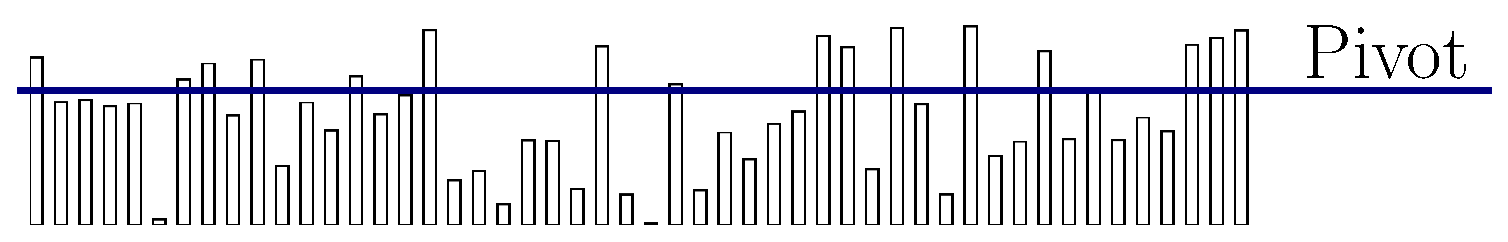
\includegraphics[width=\linewidth]{imgs/partitionDefn/partitionDefn1Ann.eps}
  {\color{blue} An array partitioned relative to the pivot value:}

  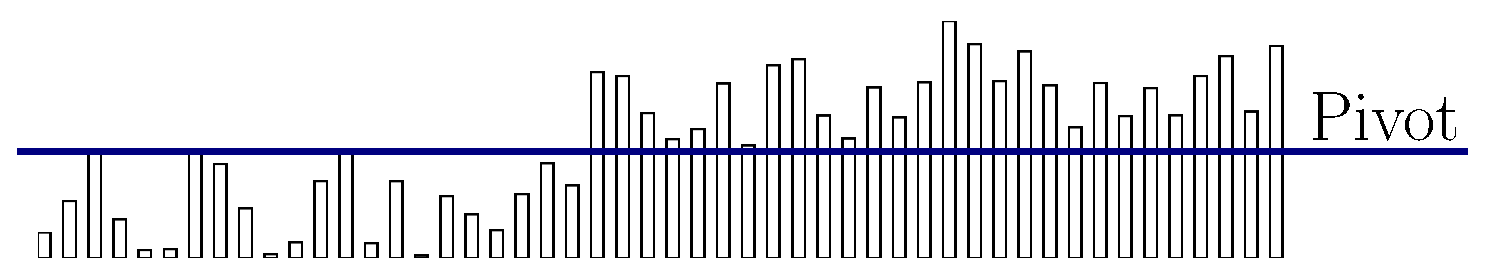
\includegraphics[width=\linewidth]{imgs/partitionDefn/partitionDefn2Ann.eps}
\end{block}
\begin{block}{\Huge What is A Parallel Algorithm?}
  \justifying
  \Huge
  \textbf{Explanation:} Whereas a typical (i.e. serial) algorithm runs on a single processor, a \emph{parallel algorithm} runs on $p \geq 1$ processors.

  \textbf{Example:} Many tasks have parts that can be performed concurrently; such tasks can be performed faster with parallel computing.

  {\color{blue} Program execution in serial and in parallel }

  \centering
  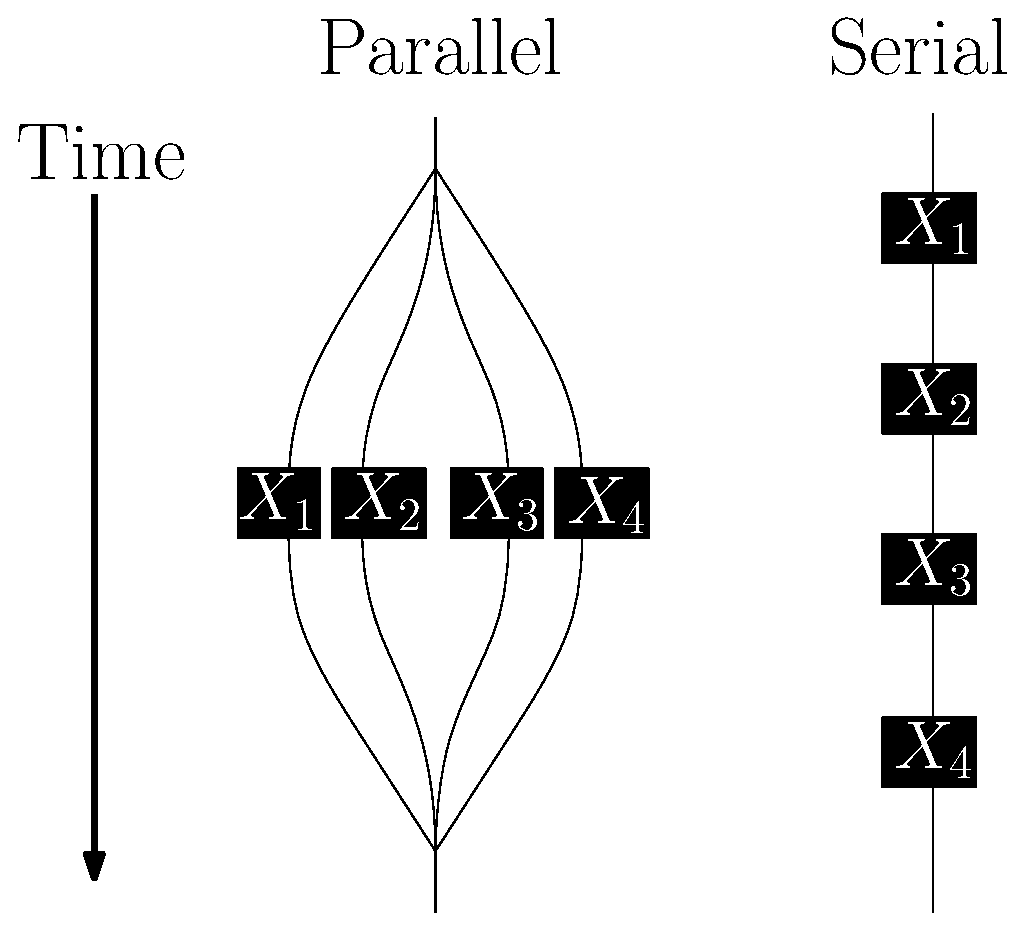
\includegraphics[width=0.6\linewidth]{imgs/parallelForLoop/serialParallelComparison.eps}
\end{block}
\begin{block}{\Huge What is Cache Efficiency?}
  \justifying
  \Huge
  \textbf{Explanation:} \emph{Cache} is a small part of memory that can be accessed much faster than ordinary RAM. When data is already loaded into Cache a program can rapidly access it; this is called a \emph{cache hit}. When data needed by a program isn't in cache it must be loaded into cache; this is called a \emph{cache miss}, and takes time. \\
  \textbf{Remark:} An algorithm with very few cache misses is \emph{Cache Efficient}; cache efficiency leads to faster performance in practice.\\
  \textbf{Factors in Cache-Efficiency:}
  \begin{itemize}
    \item Perform low number of passes over the data
    \item Don't use extra memory, i.e. are \emph{In-Place}
    \item Deal with elements that are close in memory together
  \end{itemize}
\end{block}

\begin{block}{\Huge Previous Work on the Partition Problem}
  \justifying
  \Huge
  The ``Standard Algorithm" is {\color{darkgreen} theoretically optimal with span $O(\log n)$,} {\color{red} but slow in practice due to poor cache behavior.}

  The {\color{darkgreen}fastest algorithms in practice} {\color{red}lack theoretical guarantees}
	\begin{itemize}
		\item Lock-based and atomic-variable based algorithms\\ \citefont{[Michael Axtmann, Sascha Witt, Daniel Ferizovic, and Peter Sanders, 2017; Philip Heidelberger, Alan Norton, and John T. Robinson, 1990; Philippas Tsigas and Yi Zhang, 2003]}\\
      {\color{red} Not Exclusive Read/Write Memory}
		\item The Strided Algorithm\\ \citefont{[Francis and Pannan, 92; Frias and Petit, 08]}\\ 
      {\color{darkgreen}No locks or atomic-variables,} {\color{red}but no bound on span}
	\end{itemize}
	\vspace{0.2cm}

\end{block}
  \end{column}

  \begin{column}{0.01\linewidth}
  \end{column}

  \begin{column}{0.5\linewidth}
\begin{block}{\Huge Our Research Question}
  \justifying
  \Huge Can we create an algorithm with \emph{theoretical guarantees} that is \emph{fast in practice}?
\end{block}

\begin{block}{\Huge Result}
  \justifying
  \Huge We created the \emph{Smoothed Striding Algorithm}. \\
  Key Features:
	\begin{itemize}
		\item linear work and polylogarithmic span \\
			{\color{blue} (like the Standard Algorithm)\\}
		\vspace{0.15cm}
		\item fast in practice \\
			{\color{blue} (like the Strided Algorithm)\\}
	\vspace{0.15cm}
		\item theoretically optimal cache behavior \\
			{\color{blue} (unlike any past algorithm)}
	\end{itemize}
\end{block}

\begin{block}{\Huge Smoothed Striding Algorithm}
  \Huge
	Logically partition the array into chunks of adjacent elements.
	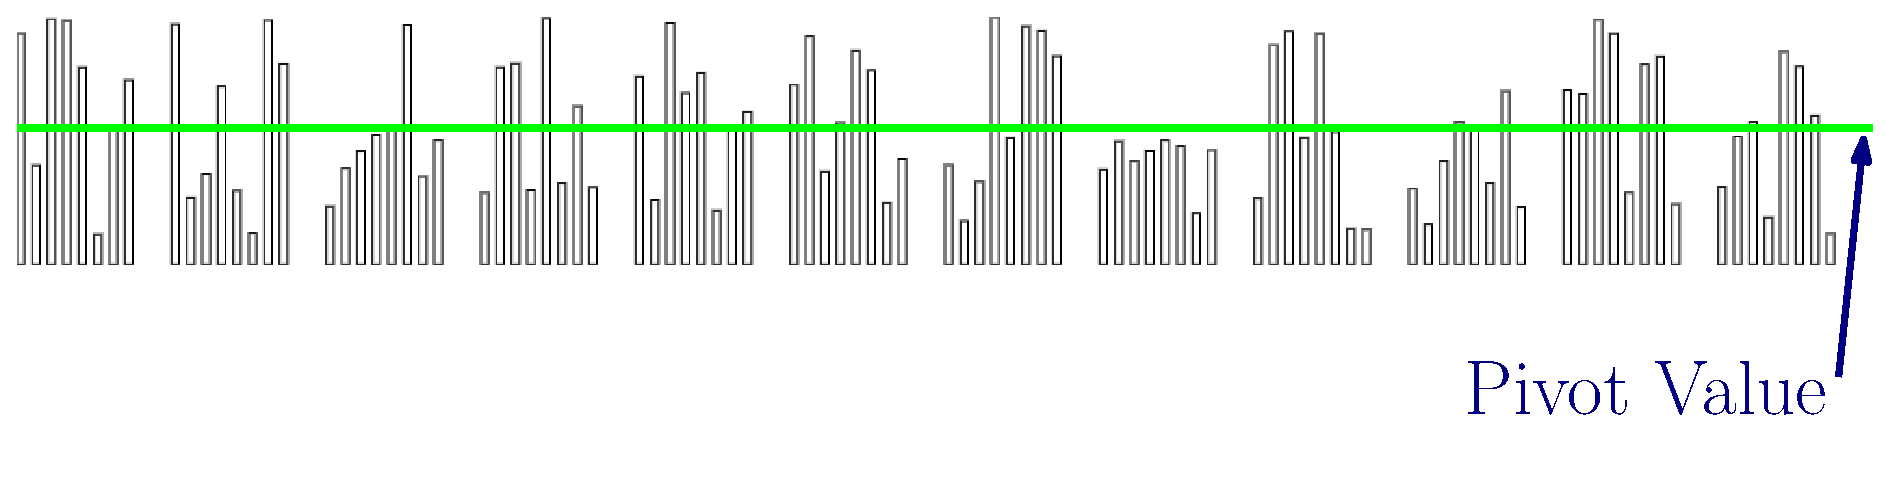
\includegraphics[width=\linewidth]{imgs/smoothedStridingAlgSim/sim1.eps}
	Form groups $U_i$ that contain a random element from each chunk. \\
  {\color{blue}This randomization step was one of our key insights; it guarantees that the $U_i$'s have similar compositions regardless of the input.}
	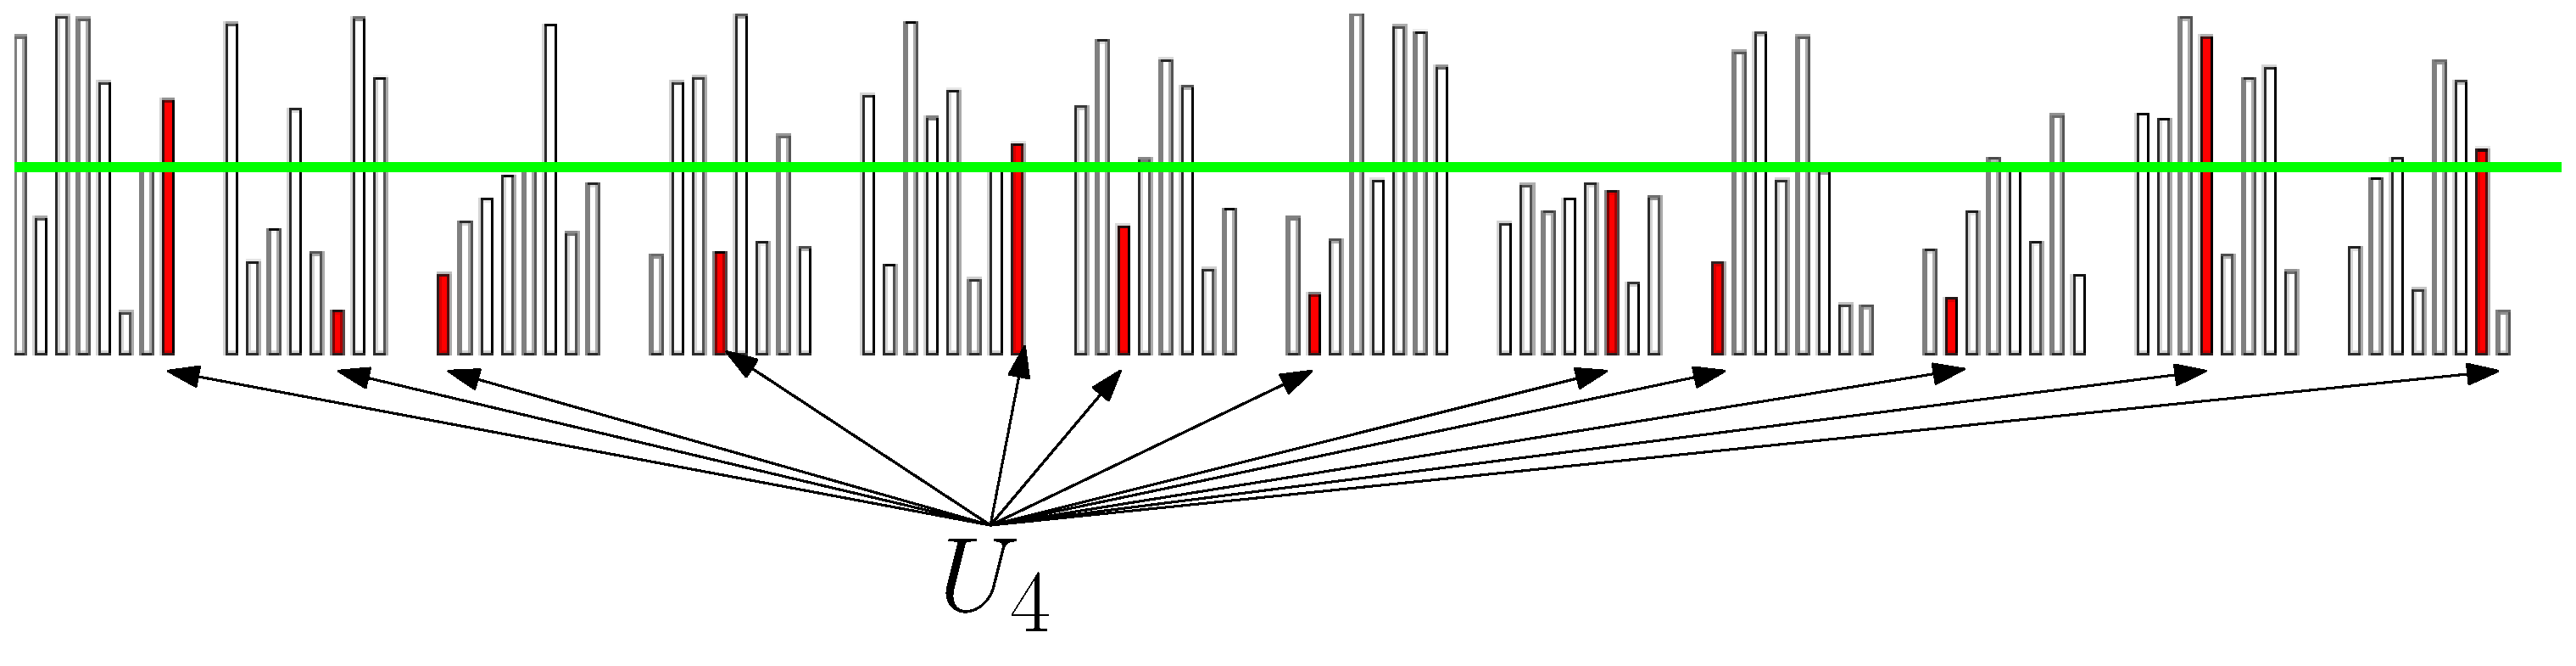
\includegraphics[width=\linewidth]{imgs/smoothedStridingAlgSim/sim2.eps}
	Perform serial partitions on each $U_i$ in parallel over the $U_i$'s. \\
  This step is highly parallel.
	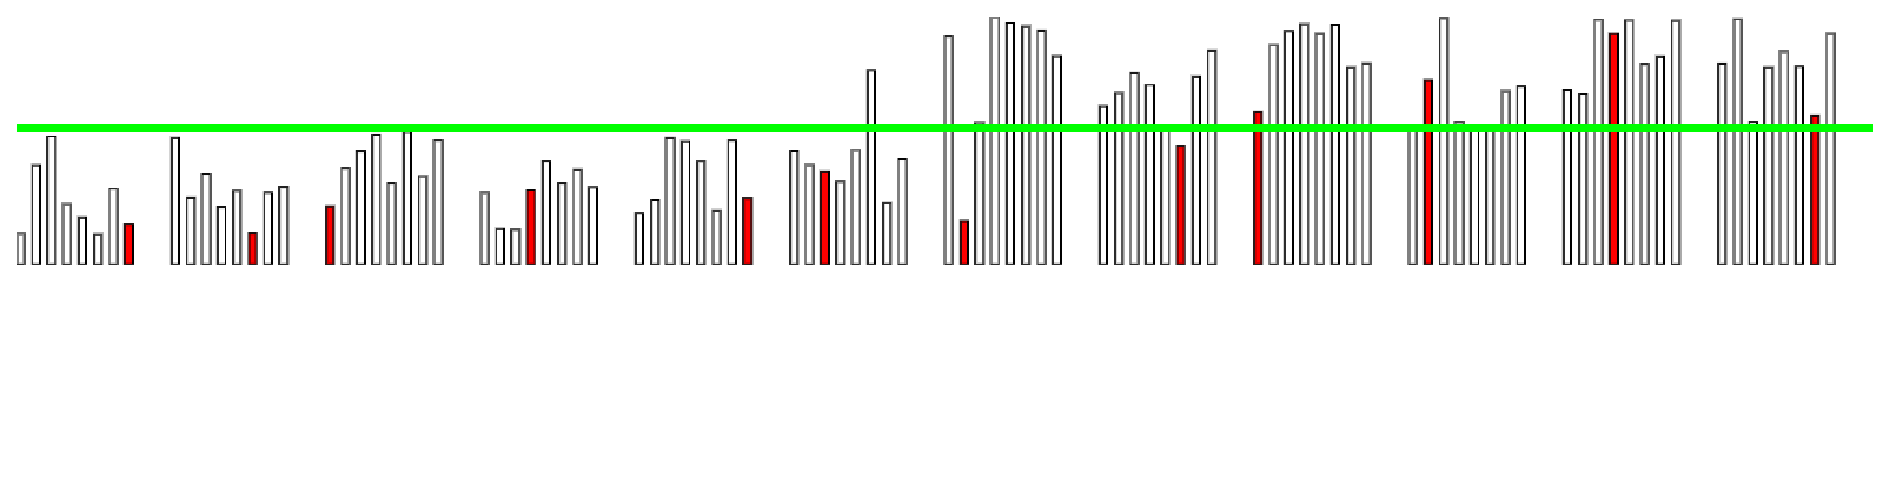
\includegraphics[width=\linewidth]{imgs/smoothedStridingAlgSim/sim3.eps}
  Define $v_i = $ index of first element greater than the pivot in $U_i$. 
	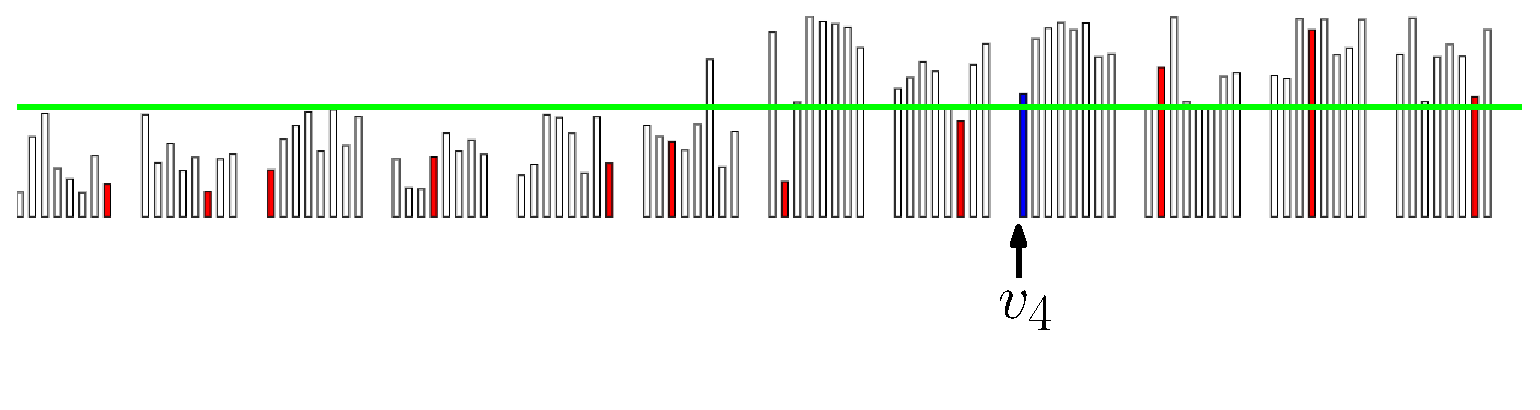
\includegraphics[width=\linewidth]{imgs/smoothedStridingAlgSim/sim35.eps}
  Identify leftmost and rightmost $v_i$. Note that $A[k] \le \text{pivot}$ for all $k < v_{\min}$, and $A[k] > \text{pivot}$ for all $k \ge v_{\max}$.
	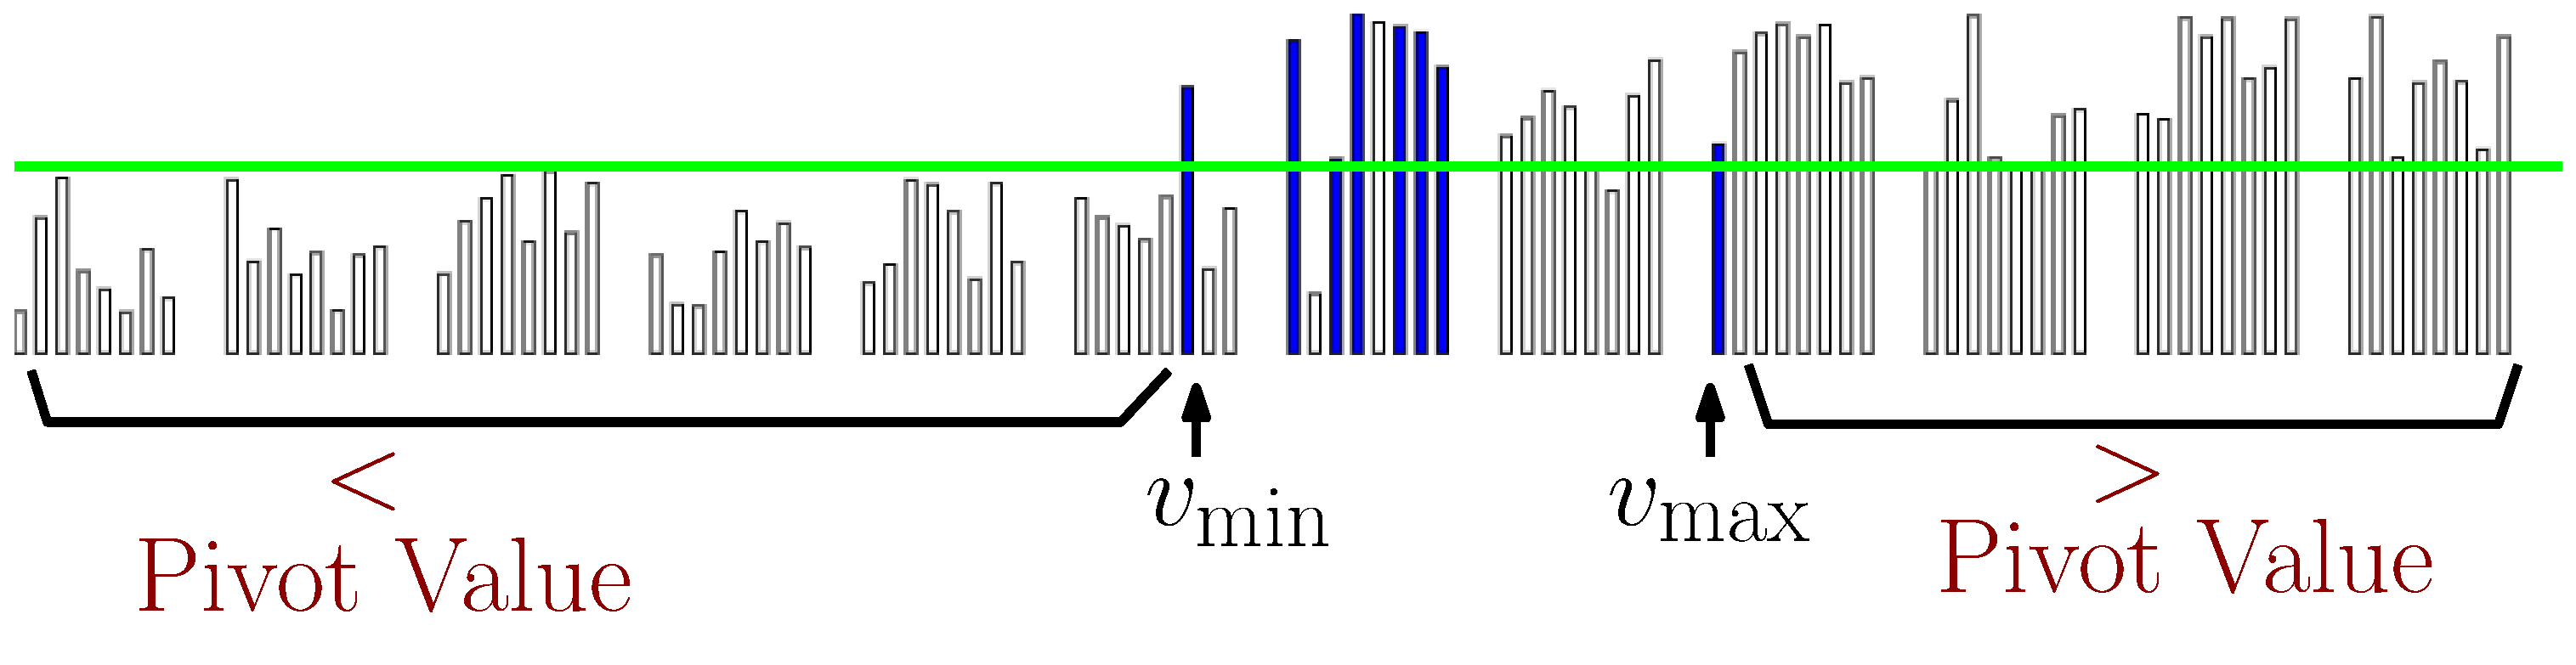
\includegraphics[width=\linewidth]{imgs/smoothedStridingAlgSim/sim4.eps}
	Recursively partition the subarray.\\
  {\color{blue}This step was previously impossible; adding randomization enables this step, which enables our algorithm's low span. }
	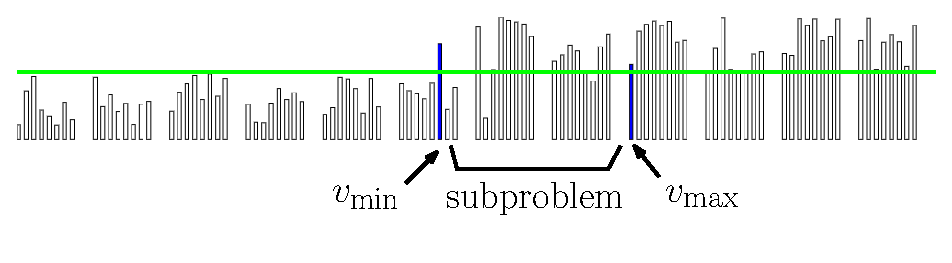
\includegraphics[width=\linewidth]{imgs/smoothedStridingAlgSim/sim45.eps}
\end{block}

  \end{column}
  \begin{column}{0.02\linewidth}
  \end{column}

\end{columns}
\end{frame}
\end{document}

